\section{Methodology}
The proposed methodology follows a pipeline-oriented design intended to transform sparse, unstructured primary-care data into safe and interpretable medication recommendations. The architecture is organized into four principal phases: Data Acquisition and Preprocessing, Patient Representation Learning, Recommendation Logic and Safety Filtering, and Interpretability Mapping.

\subsection{Data Acquisition and Preprocessing}
The system ingests clinical inputs which, in an outpatient context, primarily consist of short free-text symptom descriptions alongside basic structured attributes including age, sex, and documented comorbidities.
\begin{itemize}
    \item \textbf{Text Normalization:} To address the orthographic and lexical noise characteristic of primary-care notes, spell correction is applied and medical abbreviations are expanded to their full forms (e.g., ``SOB'' to ``Shortness of Breath'').
    \item \textbf{Medical Entity Extraction:} Identified symptoms are mapped to standardized medical ontologies---specifically SNOMED-CT or ICD-10---via a Named Entity Recognition (NER) layer, ensuring semantic consistency across heterogeneous inputs.
\end{itemize}

\subsection{Patient Representation Learning}
A multi-modal embedding strategy is adopted to capture the full clinical context of a patient encounter.
\begin{itemize}
    \item \textbf{Symptom Encoding ($E_s$):} A lightweight transformer-based encoder (Clinical DistilBERT) processes the normalized symptom text to produce a dense semantic vector. This formulation captures the nuance of patient-reported complaints while avoiding the inference latency associated with larger language models.
    \item \textbf{Feature Fusion:} Structured demographic attributes and categorical comorbidity indicators are encoded through a multi-layer perceptron (MLP) and concatenated with the symptom embedding $E_s$. The resulting joint representation, $P_v$, constitutes a unified encoding of the patient state for a given encounter.
\end{itemize}

\subsection{Recommendation Logic and Safety Filtering}
The recommendation task is framed as a multi-label classification problem, in which the model estimates the probability of each of $N$ candidate drug classes being appropriate for the patient.
\begin{itemize}
    \item \textbf{Multi-Label Head:} The fused patient representation $P_v$ is passed through a sigmoid output layer to produce per-class probabilities. To account for statistical dependencies between co-prescribed medications, a label-correlation regularizer is incorporated during training.
    \item \textbf{DDI-Aware Safety Filter:} Candidate recommendations are subsequently evaluated by a graph-based safety filter constructed from established drug--drug interaction (DDI) databases, including DrugBank. Where the proposed combination exceeds a defined interaction risk threshold, the safety layer either penalizes the offending candidate in the ranking or surfaces a clinician-facing override alert.
\end{itemize}

\subsection{Interpretability and Feedback}
To support clinical trust and adoption, the system produces dual-layered explanations accompanying each recommendation.
\begin{itemize}
    \item \textbf{Saliency Mapping:} SHAP (SHapley Additive exPlanations) values are computed to identify the specific symptom tokens that contributed most substantially to each recommendation, providing token-level attribution over the input text.
    \item \textbf{Safety Rationales:} For any flagged interaction, the system generates a knowledge-graph trace articulating the pharmacological basis of the conflict (e.g., ``Drug A and Drug B both inhibit enzyme CYP3A4''), providing a transparent and clinically grounded rationale for the safety alert.
\end{itemize}

\begin{figure}
    \centering
    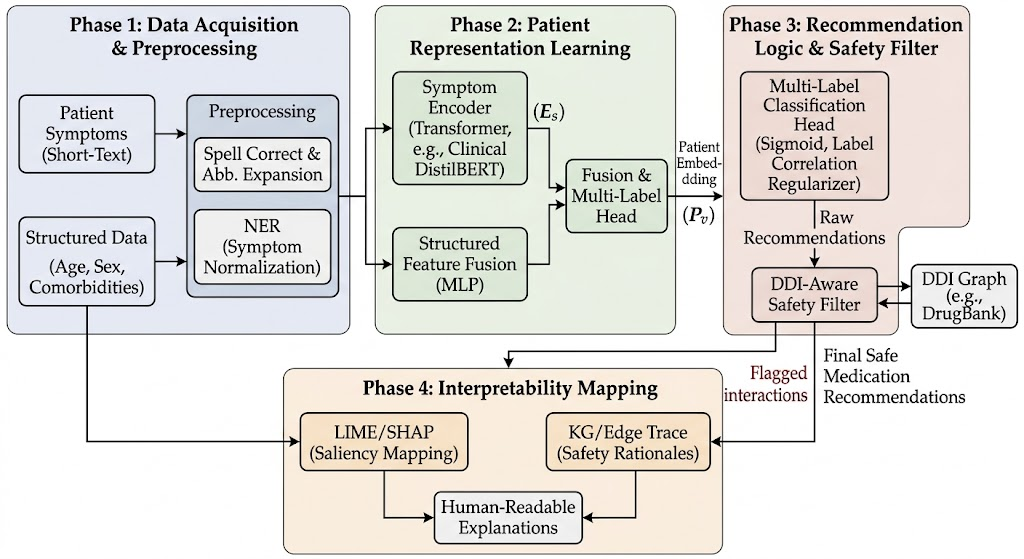
\includegraphics[width=\linewidth]{figures/architecture.png}
    \caption{Architecture diagram detailing the four phases of the proposed medication recommendation methodology, including data flow, principal modules, and the integrated safety and interpretability layers.}
    \label{fig:architecture}
\end{figure}

\subsection{Medication Recommendation Algorithm}
The complete workflow of the proposed system is formalized in Algorithm~\ref{alg:medrec}. The procedure accepts patient symptom text and structured demographic features as input, derives a unified patient representation through a combination of neural encoders, and produces medication recommendations subject to drug--drug interaction safety constraints.

\begin{algorithm}
\caption{DL\_Medication\_Recommendation\_System}
\label{alg:medrec}
\begin{algorithmic}[1]
\REQUIRE Patient symptom text $S$, structured data $D$ (age, sex, comorbidities), DDI graph $G$
\ENSURE Safe medication recommendations $M_{safe}$ and explanation report $E$
\STATE Collect patient symptom text $S$ and structured clinical attributes $D$
\STATE Apply spell correction and medical abbreviation expansion to $S$
\STATE Extract medical entities from $S$ using a Named Entity Recognition (NER) module
\STATE Map extracted entities to standardized medical terminology
\STATE Generate symptom embedding $E_s$ via a transformer-based encoder
\STATE Encode structured features $D$ through a multi-layer perceptron to obtain $E_d$
\STATE Fuse both representations to form the patient state vector:
\[
P_v = \text{Concatenate}(E_s,\; E_d)
\]
\STATE Estimate per-class medication probabilities using a sigmoid classifier applied to $P_v$
\STATE Select the top-$k$ candidates as the initial recommendation set
\STATE Apply DDI-aware safety filtering over the candidate set using interaction graph $G$
\STATE Compute SHAP-based attribution scores to generate explanation report $E$
\STATE \textbf{return} $M_{safe}$, $E$
\end{algorithmic}
\end{algorithm}

\section{Evaluation Plan}
\begin{itemize}
    \item \textbf{Data:} Synthea synthetic outpatient encounter records, augmented symptom--disease association datasets, and curated interaction data from DrugBank and TWOSIDES.
    \item \textbf{Metrics:} Diagnostic prediction performance (accuracy, macro-F1); medication recommendation quality (Jaccard index, mean average precision); DDI occurrence rate; and clinician-rated explanation utility via structured assessment.
    \item \textbf{Ablation:} Encoder ablation studies, safety-layer removal experiments, and explanation fidelity evaluations to isolate the contribution of each architectural component.
\end{itemize}
